\chapter{Causal Analysis of Theme and Sentiment on Political Ideology Classification}
\label{ch:causal-inference}

\section{Background and Motivation}
\label{sec:causal-background}

Substantial research has been conducted examining sentiment and tone analysis within the domain of political discourse and stance detection \citep{smirnova2017ideology, bhatia2018topic, bestvater2023sentiment}.
\citet{smirnova2017ideology} specifically investigated how the sentiment on the topics of Russia and Islam in New York Times articles changed after the annexation of Crimea in 2014, and 9/11, respectively. They found that articles with negative sentiment towards these topics increased significantly after these events, suggesting a correlation between sentiment and ideological framing in media coverage in this case. While \citet{bestvater2023sentiment} demonstrate that sentiment or tone alone is not a perfect predictor of ideological stance, their empirical investigation of tweets concerning political topics reveals that in specific contexts, there exists a notable correlation between sentiment and political alignment. Additionally, our findings presented in Section~\ref{sec:continued-pretraining} demonstrate that incorporating thematic and tonal signals during the pre-training phase yields statistically significant improvements in overall model performance.

A fundamental characteristic of contemporary news media is the differential framing of identical events based on outlet political orientation. Table~\ref{fig:khalil} presents a compelling illustration from AllSides, examining coverage of activist Mahmoud Khalil's arrest by outlets with contrasting political leanings. This case study reveals systematic differences in both lexical choice and sentiment attribution across topic categories.

The Associated Press coverage demonstrates positive sentiment toward \textit{Pro-Palestine Protests} through language such as "filled the lobby," while expressing negative sentiment toward \textit{Deportations} via phrases like "denounce immigration arrest." In contrast, the Fox News article exhibits positive sentiment toward \textit{Israel} by characterizing Khalil as an "anti-Israel activist," while framing \textit{Pro-Palestine Protests} negatively through the use of "occupied the lobby." 

This systematic variation in topic-specific sentiment attribution serves as a reliable indicator of underlying authorial and editorial ideological stance. Furthermore, a comparative analysis of headline construction reveals distinct rhetorical strategies: the Associated Press employs the relatively negative term "flood" alongside an explicit statement of purpose ("demand the activist's release"), whereas Fox News utilizes the more charged term "occupy" without contextualizing the protesters' objectives. These linguistic choices reflect the outlets' respective ideological orientations and demonstrate how sentiment and framing may operate as proxies for political stance.

\begin{table}[h!]
    \centering
    \begin{tabular}{p{2cm}|p{4cm} | p{4cm}}
\toprule
 &  Associated Press  & Fox News \\
 \midrule
topic tags &  Pro-Palestine Protests, Donald Trump, Israel, Deportations &  Pro-Palestine Protests, Donald Trump, Israel, Deportations \\
\midrule
title & Jewish protesters \textcolor{blue}{flood} Trump Tower’s lobby to demand the Columbia University activist’s release & Protesters supporting Mahmoud Khalil \textcolor{blue}{occupy} Trump Tower lobby \\
\midrule 
summary & 

\textcolor{blue}{Demonstrators} from a Jewish group filled the lobby of Trump Tower on Thursday to denounce the \textcolor{blue}{immigration arrest} of Mahmoud Khalil, a \textcolor{blue}{pro-Palestinian activist} who helped lead protests against Israel at Columbia University.

The \textcolor{blue}{Jewish Voice for Peace protesters}, who carried banners and wore red shirts reading “Jews say stop arming Israel,” chanted “Bring Mahmoud home now!”
 & 

About 150 \textcolor{blue}{protesters supporting Mahmoud Khalil} occupied the lobby area of Trump Tower on Manhattan's Fifth Avenue on Thursday, calling for the release of the \textcolor{blue}{anti-Israel activist} who was \textcolor{blue}{detained} over the weekend. 

The protesters, many dressed in red, held signs reading "Free Mahmoud, Free Palestine" and "Fight Nazis Not Students." The protesters were also chanting the common "Free, free Palestine" slogan. \\
\bottomrule
\end{tabular}
\caption{Allsides reporting on the Khalil arrest. Charged words indicating sentiment or stance are highlighted in blue.}
\label{fig:khalil}
\end{table}

However, a critical limitation persists both in our investigation and in the broader literature: the distinction between causal and correlational relationships remains unclear. Furthermore, there has been limited research examining the causal relationship between textual attributes and perceived political ideology. Such causal analysis is crucial for several reasons. First, by analyzing the causal links between theme, tone, and ideology within our human-annotated dataset, we can begin to identify which topics tend to be more or less polarizing, i.e., carry stronger ideological signals, and how these patterns evolve over time.  Second, by applying similar causal analysis to both our classifier outputs and large language model results, we can identify systematic differences in classification patterns between these systems and, critically, detect spurious patterns that automated classification systems may erroneously capture.

In the rest of this chapter, we outline a framework for conducting causal inference analysis on our dataset and model outputs. We present a methodology, including causal graphs and structural equation modeling, to elucidate the relationships between thematic content, tonal attributes, and ideological classification. By establishing a clearer understanding of these causal relationships, we aim to enhance the interpretability and reliability of political ideology classification systems.

\section{Methodology for Causal Inference}
\label{sec:causal-methodology}
\subsection{Causal Diagram and Variable Definitions}

To investigate the causal relationships between thematic content, tonal attributes, and ideological classification, we propose a causal diagram (Figure~\ref{fig:causal_diagram}) that captures the hypothesized dependencies among these variables. 

We define the following variables for our analysis:
\begin{itemize}
    \item $X$: (text) this represents the full text of the article parsed from the publishing source.
    \item $T$: (topic tags) this represents the topic tags assigned by Allsides (e.g. Politics, Government Efficiency, Foreign Affairs, Government Funding).
    \item $F$: (sentiment) This will be inferred from the article using an LLM.
    \item $Y$: (ideology) represents the political ideology of the article as tagged by AllSides.
\end{itemize}

The causal diagram serves as a fundamental tool for formalizing our theoretical understanding of the data-generating process and identifying the appropriate statistical methods for causal inference. By explicitly representing the assumed causal structure, the diagram enables us to determine which variables must be controlled for to obtain unbiased estimates of causal effects and to identify potential sources of confounding.

\begin{figure}[h]
    \centering
    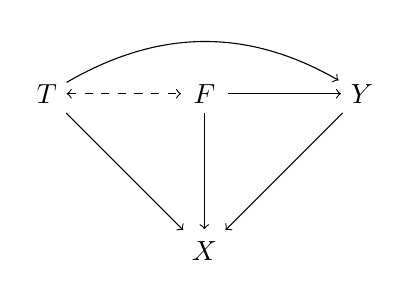
\begin{tikzpicture}[->,shorten >=1pt,auto,node distance=2cm]
      \tikzstyle{every state}=[]
    
      \node(text) {$X$};
      \node(sentiment) [above of=text] {$F$} edge [->] (text);
      \node(ideology) [right of=sentiment] {$Y$} edge [<-] (sentiment) edge [->] (text);
      \node(topic) [left of=sentiment] {$T$} edge [->] (text) edge [->, bend left] (ideology) edge [<->, dashed] (sentiment);
    \end{tikzpicture}
    \caption{Causal Diagrams}
    \label{fig:causal_diagram}
\end{figure}

In the causal diagram in figure \ref{fig:causal_diagram}, we aim to highlight the relationships between the variables as we see them interacting in the real world. The directional arrows represent hypothesized causal relationships between variables, where the arrow points from the cause to the effect. For instance, the arrow from $Y$ (ideology) to $X$ (text) indicates that political ideology causally influences the content and framing of news articles. Similarly, the arrow from $F$ (sentiment) to $X$ suggests that the sentiment toward particular topics shapes how those topics are discussed in the text. The bidirectional dashed arrow between $T$ (topic) and $F$ (sentiment) represents a more complex relationship where these variables may mutually influence each other, capturing that certain topics may inherently evoke particular sentiments, while prevailing sentiment patterns may influence which topics receive coverage. This bidirectional relationship acknowledges the potential for simultaneous causation and suggests that simple unidirectional causal assumptions may be insufficient to capture the full complexity of this relationship.


The variables in our causal model expand substantially during experimental implementation, with individual nodes representing hundreds or thousands of distinct variables due to the dimensionality of our data. We illustrate this expansion in Figure~\ref{fig:causal3}, where each sentiment variable $F$ represents a distinct sentiment dimension corresponding to a specific topic tag.
We maintain that the fundamental relationship structure \textit{between} variables adheres to the patterns illustrated in Figure~\ref{fig:causal_diagram}, despite this dimensional expansion; we simply assert that relationships \textit{within} variables change. Given that our research is focused on how sentiment expressed toward one topic may mediate the effects of sentiment toward another topic, our experimental design designates a specific sentiment variable as the treatment effect, while all other sentiment variables are treated as potential mediators in the causal pathway. 

\begin{figure}[h!]
  \centering
  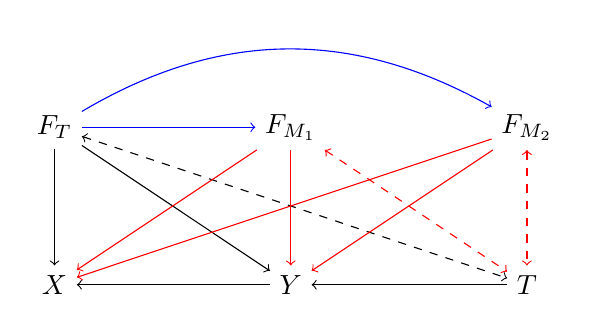
\begin{tikzpicture}[->,auto]
    % Top row: the three F’s
    \node (FT)   at (0,0)   {$F_{T}$};
    \node (FM1)  at (3,0)   {$F_{M_1}$};
    \node (FM2)  at (6,0)   {$F_{M_2}$};

    % Bottom row: the three observed variables
    \node (Xabs) at (0,-2)  {$X$};
    \node (Y)    at (3,-2)  {$Y$};
    \node (T)    at (6,-2)  {$T$};

    % Edges from F_T
    \draw[->]           (FT) -- (Y);
    \draw[->]  (FT) -- (Xabs);
    \draw[<->, dashed]  (FT) -- (T);

    % Edges from X_abs and T to Y
    \draw[<-]           (Xabs) -- (Y);
    \draw[->]  (T) to (Y);

    % Edges for F_{M_1}
    \draw[->, red]             (FM1) -- (Y);
    \draw[->, red]    (FM1) -- (Xabs);
    \draw[<->, dashed, red]    (FM1) -- (T);
    \draw[<-, blue]            (FM1) -- (FT);

    % Edges for F_{M_2}
    \draw[->, red]             (FM2) -- (Y);
    \draw[->, red]    (FM2) -- (Xabs);
    \draw[<->, dashed, red]    (FM2) -- (T);
    \draw[<-, blue, bend right] (FM2) to (FT);
  \end{tikzpicture}
  \caption{Experimental Set Up: Sentiments as mediators}
  \label{fig:causal3}
\end{figure}

To conduct rigorous causal inference, it is essential to clearly define the role of each variable in our analysis. Our central causal question examines the effect of sentiment toward a particular topic on political ideology classification. We operationalize this question through the following variable assignments:

\paragraph{Treatment Variable ($F_T$):} The sentiment expressed toward a specific topic of interest (e.g., sentiment toward "Immigration" or "Healthcare"). This represents the causal variable whose effect we seek to estimate.

\paragraph{Outcome Variable ($Y$):} The political ideology classification (Left/Center/Right) assigned to the article. This represents the dependent variable that we hypothesize is causally influenced by topic-specific sentiment.

\paragraph{Mediator Variables ($F_{M_1}, F_{M_2}, \ldots$):} The sentiments expressed toward all other topics present in the article. These variables lie on the causal pathway between the treatment sentiment and ideology classification, as sentiment toward one topic may influence sentiment expression toward related topics, which in turn affects overall ideology perception. The blue arrows in Figure~\ref{fig:causal3} illustrate these mediating relationships.

\paragraph{Confounder Variables:} Variables that influence both the treatment and outcome, potentially creating spurious associations. In our model, $T$ (topic presence) serves as a confounder, as the presence of certain topics may simultaneously influence both the sentiment expressed toward those topics and the overall ideology of the article. Similarly, $X$ (text content) acts as a collider, being influenced by both sentiment and ideology.

To ensure valid causal inference, we restrict our analysis to articles that contain the treatment topic of interest. This design choice prevents invalid comparisons between articles with and without the relevant topic, as sentiment toward a topic can only be meaningfully measured when that topic is actually discussed. This experimental design enables us to estimate Average Treatment Effects (ATE) and Conditional Average Treatment Effects (CATE). The ATE quantifies the average causal impact of sentiment toward a specific topic on political ideology classification across all articles in our sample, providing a population-level estimate of this relationship. CATE analysis extends this by examining how treatment effects vary across different subgroups or conditions, such as presence of other specific topics. This heterogeneity analysis is particularly valuable for understanding whether sentiment-ideology relationships are universal or contingent upon contextual factors. This framework also allows us to analyze the Natural Direct Effect (NDE) of treatment sentiment on ideology, as well as the Natural Indirect Effects (NIE) mediated through sentiments toward other topics, providing insights into how topic-specific sentiment patterns contribute to overall ideological classification.

\subsection{Data Collection}
We use the AllSides extended dataset described in Section~\ref{sec:dataset} as the basis for our causal inference analysis. To extract sentiment variables ($F$), we employ a two-step process to analyze the full text of each article ($X$) and generate sentiment scores for each topic tag ($T$) associated with the article:

\begin{enumerate}
\item Entity and Sentiment Analysis:
\begin{itemize}
    \item Named entities and key concepts were extracted from the text corpus.
    \item The \texttt{llama-3.3-70b-versatile} model was deployed to analyze sentiment polarity for each identified entity.
    \item This particular large language model was selected for its superior capacity to detect subtle sentiment variations and contextual nuances compared to smaller alternatives.
    \item A continuous sentiment scale was employed, ranging from $-1.0$ (indicating strong negative sentiment) to $+1.0$ (indicating strong positive sentiment).
\end{itemize}

\item Entity-to-Topic Tag Association Analysis:
\begin{itemize}
    \item Extracted entities were processed through the \texttt{llama3-70b-8192} model to quantify their association strength with predefined thematic tags.
    \item The model demonstrated good temporal and conceptual discernment, avoiding spurious correlations based merely on chronological coincidence. For instance, it correctly distinguished between terrorism as a broader concept and specific incidents like the March 2019 Christchurch shooting when deciding to assign entity "shooting" to topic "Christchurch" or topic "Violence".
    \item Entity sentiment scores were aggregated by tag to create cumulative sentiment profiles for each topic.
\end{itemize}
\end{enumerate}

\subsection{Experimental Design}
\label{sec:experimental-design}

To ensure fair comparison across annotation sources, we perform our analysis exclusively on the test set of the AllSides dataset. To identify the topical structure underlying this test set, we applied the Louvain community detection algorithm to a co-occurrence graph of topic tags. In this graph construction, nodes represent individual topic tags, while edges capture tag co-occurrence relationships weighted by the frequency with which tag pairs appear together within articles. To accommodate articles containing only a single topic tag, we incorporated self-loops that allow isolated tags to form their own communities. This approach yielded a modularity score of 0.498 across 12 distinct communities, with community sizes ranging from 1 to 199 tags and an average community size of 101.0 tags. 

\begin{table}[h]
    \centering
    \begin{tabular}{lcc}
    \toprule
    \textbf{Topic Tag} & \textbf{Articles} & \textbf{Community} \\
    \midrule
    politics & 756 & 2 \\
    donald\_trump & 712 & 11 \\
    world & 503 & 4 \\
    elections & 451 & 11 \\
    white\_house & 444 & 2 \\
    \bottomrule
    \end{tabular}
    \caption{Top Five Topic Tags by Frequency (Test Set)}
    \label{tab:top-tags}
\end{table}

Given the focused scope of our test set analysis, we concentrate our experimental design on the five most frequent topic tags as shown in Table~\ref{tab:top-tags}. This selection ensures sufficient statistical power while capturing cross-community relationships between the communities. As we see in Figure~\ref{fig:louvain}, these top five tags span three distinct communities with strong inter-community connections: political figures and electoral processes (Community 11: \textit{donald\_trump}, \textit{elections}), institutional politics (Community 2: \textit{politics}, \textit{white\_house}), and international affairs (Community 4: \textit{world}). This distribution enables us to investigate how sentiment toward topics from different thematic domains interacts to influence ideological classification.

\begin{figure}[h!]
    \centering
    \includegraphics[width=0.7\textwidth]{sections/images/louvain_communities.png}
    \caption{Louvain Community Detection on Topic Tag Co-Occurrence Graph for Top Five Tags}
    \label{fig:louvain}
\end{figure}

Our primary experiment examines the bidirectional relationship between sentiment toward \textit{donald\_trump} (Community 11) and sentiment toward \textit{politics} (Community 2) in shaping ideological classification. We investigate two competing hypotheses: (1) sentiment toward Donald Trump as a political figure drives general political sentiment, which then influences ideology classification, versus (2) broader political sentiment shapes perceptions of Donald Trump, with Trump-specific sentiment serving as the mediator to ideology. This analysis employs both NIE/NDE decomposition and bidirectional mediation modeling to determine the dominant causal pathway and quantify the relative strength of direct versus mediated effects.

Building on the Trump-politics relationship, we examine whether the mediation pattern generalizes across communities by testing whether institutional political topics (Community 2: \textit{politics}, \textit{white\_house}) systematically mediate the effects of political figure sentiment (Community 11: \textit{donald\_trump}, \textit{joe\_biden}) on ideological classification. We estimate CATE for different combinations of Community 11 and Community 2 sentiment variables, testing the hypothesis that institutional framing consistently moderates the impact of personalized political sentiment. This analysis reveals whether the Trump-politics dynamic represents a general structural relationship between individual political figures and institutional politics.

We conduct the experimental analysis across three annotation sources, enabling comparison of causal mechanisms across different classification approaches:

\begin{enumerate}
    \item Gold Standard Human Annotations: Manual ideological classifications provided by the AllSides human annotators, serving as our ground truth baseline for causal relationships.
    
    \item Fine-tuned Classifier: Predictions from the best-performing fine-tuned classifier model introduced in Section~\ref{sec:continued-pretraining}, representing automated classification based on continued pre-training approaches.
    
    \item Fine-tuned GPT-4o-mini: Predictions from the fine-tuned GPT-4o-mini model presented in Section~\ref{sec:llm-finetuning}, representing large language model-based classification approaches.
\end{enumerate}

This comparative framework allows us to examine whether the causal relationships we identify are consistent across different classification paradigms or whether they vary systematically between human judgment, traditional machine learning approaches, and large language model-based systems.
